
\documentclass[a4paper,twoside]{refart}

%\usepackage{fancyhdr}
%\usepackage{makeidx}
%\usepackage{amssymb}
%\usepackage{url}
\usepackage{longtable}
%\usepackage{multicol}
%\usepackage{graphics}
\usepackage{graphicx} 
%\usepackage{subfigure}

\usepackage{gensymb}
\usepackage[stable]{footmisc}
\usepackage{multirow}

\usepackage{hyperref}
\hypersetup{
    colorlinks,
    citecolor=black,
    filecolor=black,
    linkcolor=black,
    urlcolor=blue
}

\usepackage{listings} % Required for inserting code snippets
\usepackage[usenames,dvipsnames]{color} % Required for specifying custom colors and referring to colors by name

\definecolor{highlight}{RGB}{255,251,204} % Code highlight color

\lstdefinelanguage{sms}
{morekeywords={code,gprs,setup,fix,apn,user,pass,srv,port,vref,err,set},
sensitive=false,
morestring=[b]",
}

\lstset{
language=sms, % Detects keywords, comments, strings, functions, etc for the language specified
backgroundcolor=\color{highlight}, % Set the background color for the snippet - useful for highlighting
%basicstyle=\footnotesize\ttfamily, % The default font size and style of the code
basicstyle=\ttfamily, % The default font size and style of the code
breakatwhitespace=false, % If true, only allows line breaks at white space
breaklines=true, % Automatic line breaking (prevents code from protruding outside the box)
captionpos=b, % Sets the caption position: b for bottom; t for top
deletekeywords={}, % If you want to delete any keywords from the current language separate them by commas
%escapeinside={\%}, % This allows you to escape to LaTeX using the character in the bracket
firstnumber=1, % Line numbers begin at line 1
frame=single, % Frame around the code box, value can be: none, leftline, topline, bottomline, lines, single, shadowbox
frameround=tttt, % Rounds the corners of the frame for the top left, top right, bottom left and bottom right positions
keywordstyle=\color{Blue}\bf, % Functions are bold and blue
morekeywords={}, % Add any functions no included by default here separated by commas
numbers=left, % Location of line numbers, can take the values of: none, left, right
numbersep=10pt, % Distance of line numbers from the code box
numberstyle=\tiny\color{Gray}, % Style used for line numbers
rulecolor=\color{black}, % Frame border color
showstringspaces=false, % Don't put marks in string spaces
showtabs=false, % Display tabs in the code as lines
stepnumber=5, % The step distance between line numbers, i.e. how often will lines be numbered
stringstyle=\color{Purple}, % Strings are purple
tabsize=2, % Number of spaces per tab in the code
}

\renewcommand*{\familydefault}{\sfdefault}
%\renewcommand*{\familydefault}{\rmdefault}
%\renewcommand*{\familydefault}{\ttdefault}
%\renewcommand*{\familydefault}{\rmdefault{ppl}}

\begin{document}
\title{gps tracking module with gprs connectivity}
\author{\url{http://www.simplex.ro}}
\date{created September 2014, revised \today}
\maketitle

\begin{abstract}
this module can be used to track goods wherever gsm signal is present. it is optimized for very low power consumption and small form factor
\end{abstract}


\tableofcontents
\newpage

\section{principles of operation}
geographic coordinates are obtained by decoding NMEA sentences received from the GPS chipset and then transmitted via the mobile phone network to a web server. the server stores the received information into a database and provides it on demand to the end-user.

cell tower identifiers are also transmitted in the same packet and this allows approximate localization when the gps signal is obstructed. when the gsm signal is missing data is being stored on the device and it's transmission will resume once connection is re-established.


\section{components used}
\subsection{software}

all the documentation, sources and hardware schematics are provided as Open Source in order to encourage further improvements by the community. the TI spy-bi-wire protocol can be used to reflash the enclosed microcontroller.

firmware is written in C and it's created to be fully non-blocking and interrupt driven. the server-side scripts are in perl and bash.

any web server can be used to receive the binary data sent from the tracker. the unpack() function present in perl, python, php will reconstruct the information and make it ready to be inserted into a database.

provided scripts have the following runtime dependencies (some are optional):

\begin{itemize}
    \item perl at least ver 5.8.2
    \item sqlite at least ver 3.0.0
    \item bash
    \item nginx
    \item fcgi
\end{itemize}

and in order to modify the software one needs:

\begin{itemize}
    \item msp430-gcc (ver 4.6.3\_p20120406 has been used)
    \item msp430-binutils (2.22\_p20120911)
    \item msp430-libc (20120716)
    \item msp430mcu (20120716)
    \item mspdebug (0.22)
\end{itemize}


\subsection{hardware}

\marginlabel{MSP430F5510 mixed signal microcontroller}
    \begin{itemize}
        \item 16bit RISC architecture with 32KB flash and 4KB of SRAM
        \item low supply voltage - 2.8V used in this implementation
        \item ultra-low power consumption // XXX
        \item 10bit ADC - both the battery voltage and input voltage levels are kept in check
        \item 4 16bit timers with interrupt generation - used to syncronize all processes
        \item real-time clock - keeps calendar data and the clock when gps signal is missing
        \item port mapping controller - allows digital functions to be switched between different ports
        \item watchdog, brown out reset - ensures the system runs in stable parameters
    \end{itemize}

\marginlabel{SIM900 quad-band GSM/GPRS engine}
    \begin{itemize}
        \item GSM 850MHz, EGSM 900MHz, DCS 1800MHz, PCS 1900MHz frequencies are supported
        \item a dedicated user-provided micro SIM is needed to connect to the mobile phone network of choice. M2M SIMs also work since voice is never used in this application.
    \end{itemize}

\marginlabel{MT3339 MediaTek GPS chipset}
    \begin{itemize}
        \item tiny gps module that can track 22 satellites at any given moment
        \item even if the module is mostly shut down to conserve power, the backup voltage is always provided thus ensuring a fast time-to-fix when started up
        \item automatic antenna switching detects external antennas
    \end{itemize}
\marginlabel{BQ24072 power path management IC}
    \begin{itemize}
        \item allows charging of the Li-Ion/LiPo cell from a USB friendly 5V source
        \item maximum charging current is limited to 300mA
    \end{itemize}
\marginlabel{FM24V10 IC}
    \begin{itemize}
        \item additional 1Mbit F-RAM for data buffering and storage
    \end{itemize}
\marginlabel{accu}
    \begin{itemize}
        \item 1 cell LiPo battery for standalone operation
    \end{itemize}

\subsubsection{absolute maximum ratings}

\begin{tabular}{ |c|c|l|c|c|c| }
    \hline
    \multicolumn{3}{|c|}{} & \multicolumn{2}{|c|}{value} & unit \\ \cline{4-6}
    \multicolumn{3}{|c|}{} & min & max & \\ \hline
    \multicolumn{1}{|c|}{\multirow{2}{*}{$V_{I}$}} & \multicolumn{1}{|c|}{\multirow{2}{*}{input voltage}} &    IN (with respect to VSS) & -0.3    & 28  & V \\ \cline{3-6}
                &                       &  VBAT (with respect to VSS)   & -0.3  & 5   & V \\ \hline
    $V_{IO}$ & \multicolumn{2}{|l|}{IO voltage thru the debug connector}                      & -0.3  & 3.1 & V \\ \hline
    $T_{stg}$   & \multicolumn{2}{|l|}{storage temperature}             & -65   & 150 & \degree C \\  \hline
    $T_{op}$   & \multicolumn{2}{|l|}{operating temperature}          & 0     & 125 & \degree C \\  \hline
\end{tabular}

Stresses above those listed in absolute maximum ratings may cause permanent damage to the device. This is a stress rating only, functional operation of the device at these or any other conditions above those indicated in the operational section of this specification is not implied. Exposure to absolute maximum rating conditions for extended periods may affect device reliability.
\newpage

\subsubsection{electrical characteristics}

\begin{tabular}{ |c|l|c|c|c|c| }
    \hline
    \multicolumn{2}{|c|}{} & \multicolumn{3}{|c|}{value} & unit \\ \cline{3-6}
    \multicolumn{2}{|c|}{} & min & typ & max & \\ \hline
    $V_{I}$ & input voltage range                      & 4.35  & 5     & 6.4  & V \\ \hline
    $I_{I}$ & input current                            & X     & X     & 1.5  & A \\ \hline
    $V_{BAT}$ & battery voltage range                  & 3.4   &       & 4.1  & V \\ \hline
    $I_{BAT}$ & battery current while discharging      & X     & X     & 2000 & mA \\ \hline
    $I_{CHG}$ & battery charging current \footnotemark &       & 0.3   &   & A \\ \hline
    $V_{IO}$ & IO voltage thru the debug connector     & 0     &       & 2.8  & V \\ \hline
\end{tabular}

\footnotetext{The charging current is configurable by changing the value of R11. See the module schematic and the bq24072 datasheet for details}

\section{connectors}
for all pin connectors, pin 1 is marked by a small triangle in the silkscreen

%\marginlabel{battery thermistor}
\begin{tabular}{ |l|p{8cm}| }
    \hline
    \multicolumn{2}{|l|}{battery thermistor} \\
    \hline
        connector & Molex 053048-0210 \\
        footprint & \begin{center} 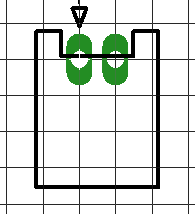
\includegraphics[height=50pt]{img/con2} \end{center} \\ \hline
        silkscreen & \verb"10KOhm ts" \\ \hline
        use & some battery packs provide this component as a charge ending protection. by default this connector is unpopulated and if it's use is required the 10K resistor located on the other side of the PCB needs to be removed \\
    \hline
    \multicolumn{2}{|l|}{pin assignments} \\
    \hline
        1   &   10K NTC thermistor \\
        2   &   10K NTC thermistor (also GND)\\
    \hline
\end{tabular}

\begin{tabular}{ |l|p{8cm}| }
    \hline
    \multicolumn{2}{|l|}{LiPo/Li-Ion 1 cell battery} \\
    \hline
        connector & Molex 053048-0210 \\
        footprint & \begin{center} 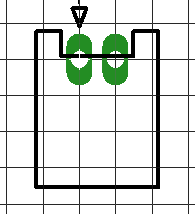
\includegraphics[height=50pt]{img/con2} \end{center} \\ \hline
        silkscreen & \verb"3.7V bat"  \\ \hline
        use & 1 cell (3.7V) rechargeable Li-Ion or Li polymer battery \\
    \hline
    \multicolumn{2}{|l|}{pin assignments} \\
    \hline
        1   &   GND \\
        2   &   +3.7V \\
    \hline
\end{tabular}

\begin{tabular}{ |l|p{8cm}| }
    \hline
    \multicolumn{2}{|l|}{5V DC input} \\
    \hline
        connector & Molex 053048-0210 \\
        footprint & \begin{center} 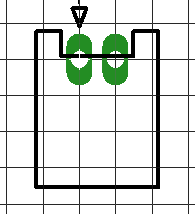
\includegraphics[height=50pt]{img/con2} \end{center} \\ \hline
        silkscreen & \verb"5V" \\ \hline
        use & 5V DC either from a USB connection or a DCDC converter. used only to charge the included batterywith a current up to 300mA \\
    \hline
    \multicolumn{2}{|l|}{pin assignments} \\
    \hline
        1   &   GND \\
        2   &   +5V \\
    \hline
\end{tabular}

\begin{tabular}{ |l|p{8cm}| }
    \hline
    \multicolumn{2}{|l|}{programming/debug connector} \\
    \hline
        connector & Molex 053048-0610 \\
        footprint & \begin{center} 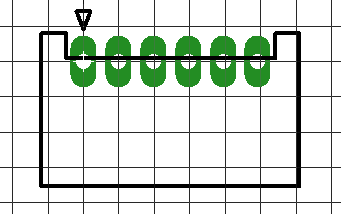
\includegraphics[height=50pt]{img/con6} \end{center} \\ \hline
        silkscreen & \verb"debug" \\ \hline
        use & pins 3-6 are used for TI's spy-bi-wire protocol in order to program or to debug the microcontroller. pins 1 and 2 can have a custom assignation \\
    \hline
    \multicolumn{2}{|l|}{pin assignments} \\
    \hline
        1   &   P4.1 - context dependant microcontroller port \\
        2   &   P4.0 - context dependant microcontroller port \\
        3   &   2.8V - VCC OUT \\
        4   &   TEST \\
        5   &   RST \\
        6   &   GND \\
    \hline
\end{tabular}

\begin{tabular}{ |l|p{8cm}| }
    \hline
    \multicolumn{2}{|l|}{gsm antenna} \\
    \hline
        connector & UFL \\
         & \begin{center} 
\includegraphics[height=40pt]{img/ufl} \end{center} \\ \hline
        silkscreen & \verb"gsm" \\ \hline
        use & it is mandatory to connect the enclosed antenna via this connector \\
    \hline
    \multicolumn{2}{|l|}{pin assignments} \\
    \hline
        shroud   &   GND \\
        center   &   signal \\
    \hline
\end{tabular}

\begin{tabular}{ |l|p{8cm}| }
    \hline
    \multicolumn{2}{|l|}{gps antenna} \\
    \hline
        connector & UFL \\
         & \begin{center} 
\includegraphics[height=40pt]{img/ufl} \end{center} \\ \hline
        silkscreen & \verb"gps" \\ \hline
        use & the gps module used provides a small patch antenna but one can improve signal reception by using an external one \\
    \hline
    \multicolumn{2}{|l|}{pin assignments} \\
    \hline
        shroud   &   GND \\
        center   &   signal \\
    \hline
\end{tabular}

\newpage
\section{usage}

\subsection{SIM cards}

below is a step-by-step guide for installing a local SIM card into the tracking module. the setup of a 'Vodafone prepay card' is shown as an example and one can adapt each step to their particular use case.

\begin{itemize}
    \item buy a SIM card. any SIM card will do: prepayed, subscription (but do keep in mind that no voice transmission will ever be used on this SIM tho), machine to machine (also known as M2M). rev1 boards use full size SIM cards, rev2 use a mini SIM form factor.
    \item obtain the associated phone number and enter it into your phone's addressbook - don't forget to also add the country prefix so you can contact the tracker while abroad. it's "+4" prefixed to the number in Romania.
    \item place the newly purchased SIM card into an actual phone
    \item if it has no initial credit, fill it with at least 5EUR
    \item make sure no PIN is set on the SIM itself
    \item disable any 'best value plan' the provider might have selected - this is easiest to do from the 'MYVodafone' entry from within the vodafone.ro website. This SIM will mostly be used to connect to the internet, and it will send a minimal number of SMS messages during the setup process. the only extra options that are needed are '100MB internet for 1 Month - 2EUR'. you can optionaly activate roaming.
    \item disable 'VOX voicemail' by calling \#\#002\#
    \item place the SIMs back into their proper locations: the newly purchased one in the tracker and your old one into the phone.
    \item while inserting the SIM into the tracker write down the last 4 IMEI digits that you see written on the SIM900 IC that is adiacent to the SIM holder.
    \item send a SMS from the phone to the tracker that contains:

\begin{lstlisting}
code 5551
\end{lstlisting}

'5551' will need to be replaced by those digits you wrote down during the previous step

    \item power on the tracker and wait. it only connects to the gsm network every 10 minutes by default and it has a 1 minute interval in which it's actively listening to incoming SMS messages. once the code is received and acknowledged you will get a 'code ok' reply on the phone. from this moment on you can send commands to the tracker.
\end{itemize}

\newpage
\subsection{SMS commands}

\begin{tabular}{ |l|p{8cm}| }
    \hline
        command & 
\begin{lstlisting}
code STRING
\end{lstlisting} \\
        action & pair a phone to the tracker.
STRING has to be the last 4 digits of the SIM900's IMEI \\ \hline
\end{tabular}


\begin{tabular}{ |l|p{8cm}| }
    \hline
        command & 
\begin{lstlisting}
gprs
\end{lstlisting} \\
        action & show APN, USER, PASSWORD that are currently used in order to authenticate for a gprs session \\ \hline
\end{tabular}


\begin{tabular}{ |l|p{8cm}| }
    \hline
    \multicolumn{2}{|l|}{} \\
    \hline
        command & 
\begin{lstlisting}
setup
\end{lstlisting} \\
        action & show a hex value containing current switches \\ \hline
\end{tabular}


\begin{tabular}{ |l|p{8cm}| }
    \hline
        command & 
\begin{lstlisting}
fix
\end{lstlisting} \\
        action & 
try to send back a GPS fix as a SMS reply \\ \hline
\end{tabular}


\begin{tabular}{ |l|p{8cm}| }
    \hline
        command & 
\begin{lstlisting}
apn STRING
\end{lstlisting} \\
        default & live.vodafone.com \\
        action & 
set the gprs apn value - max 20 char long

in case STRING is missing, an empty apn is used \\ \hline
\end{tabular}


\begin{tabular}{ |l|p{8cm}| }
    \hline
        command & 
\begin{lstlisting}
user STRING
\end{lstlisting} \\
        default & live \\
        action & 
set the gprs user  - max 20 char long

in case STRING is missing, an empty username is used  \\ \hline
\end{tabular}


\begin{tabular}{ |l|p{8cm}| }
    \hline
        command & 
\begin{lstlisting}
pass STRING
\end{lstlisting} \\
        default & vodafone \\
        action & 
set the gprs pass - max 20 char long
in case STRING is missing, an empty password is used  \\ \hline
\end{tabular}


\begin{tabular}{ |l|p{8cm}| }
    \hline
        command & 
\begin{lstlisting}
srv STRING
\end{lstlisting} \\
        default & trk.simplex.ro \\
        action & 
what server to contact in order to send the tracking data \\ \hline
\end{tabular}


\begin{tabular}{ |l|p{8cm}| }
    \hline
        command & 
\begin{lstlisting}
port STRING
\end{lstlisting} \\
        default & 80 \\
        action & 
TCP port used during connection to the server  \\ \hline
\end{tabular}


\begin{tabular}{ |l|p{8cm}| }
    \hline
        command & 
\begin{lstlisting}
vref STRING
\end{lstlisting} \\
        default & 200 \\
        action & 
STRING is a number between 190 and 210 that acts as calibration coefficient to the onboard ADC. only used if the voltage values reported by the module differ from the measured ones \\ \hline
\end{tabular}


\begin{tabular}{ |l|p{8cm}| }
    \hline
        command & 
\begin{lstlisting}
err
\end{lstlisting} \\
        action & 
shows a hex value in case there were any errors logged in the device. this value gets reset when all power is lost, when an 'err' command is replied to or after a HTTP POST packet is sent out/stored to FRAM. only used for debug  \\ \hline
\end{tabular}




ADC - analog to digital converter
M2M - machine to machine dataplan - subscription that covers SMS and data but no voice

\end{document}
